\documentclass[10pt,a4paper]{report}


\usepackage{amsmath}
\usepackage[utf8]{inputenc}
\usepackage{amsmath}
%\usepackage{unicode-math}
\usepackage{amsfonts}
\usepackage{amssymb}
\usepackage{calrsfs}
\usepackage[left=2cm,right=2cm,top=2cm,bottom=2cm]{geometry}
\usepackage[mathscr]{euscript}

\usepackage{color}

%%%%%%%%Draws Pretty Box%%%%%%%
%%%Use with \bluebox[<top pad>][<bot pad>]{<contents>}
\definecolor{myblue}{rgb}{.8, .8, 1}

\usepackage{empheq}

\newlength\mytemplen
\newsavebox\mytempbox

\makeatletter
\newcommand\bluebox{%
    \@ifnextchar[%]
       {\@bluebox}%
       {\@bluebox[0pt]}}

\def\@bluebox[#1]{%
    \@ifnextchar[%]
       {\@@bluebox[#1]}%
       {\@@bluebox[#1][0pt]}}

\def\@@bluebox[#1][#2]#3{
    \sbox\mytempbox{#3}%
    \mytemplen\ht\mytempbox
    \advance\mytemplen #1\relax
    \ht\mytempbox\mytemplen
    \mytemplen\dp\mytempbox
    \advance\mytemplen #2\relax
    \dp\mytempbox\mytemplen
    \colorbox{myblue}{\hspace{1em}\usebox{\mytempbox}\hspace{1em}}}
%%%%%%%%%%%%%%%%%%%%%%%%%%%%%%%%%%%%%%%%%%%%%

%%%%%%%%%%for writing symbol above an equality
\newcommand\xeq{\stackrel{\mathclap{\normalfont\mbox{d}}}{=}}
%%%%%%%%%%%%%%%%%%%%%%%%%%%%%%%%%%%%%%%%%%%%

%%%for drawing commutative diagrams.%%%%%%
\usepackage{tikz-cd}  
%%%%%%%%%%%%%%%%%%%%%%%%%%%%%%%%%%%%%%%%%%

%%%%%%%%%%for changing margin
\def\changemargin#1#2{\list{}{\rightmargin#2\leftmargin#1}\item[]}
\let\endchangemargin=\endlist 

\newenvironment{proof}
{\begin{changemargin}{1cm}{0.5cm} 
	}%your text here
	{\end{changemargin}
}

\newenvironment{subproof}
{\begin{changemargin}{0.5cm}{0.5cm} 
	}%your text here
	{\end{changemargin}
}
%%%%%%%%%%%%%%%%%%%%%%%%%%%%%

\begin{document}
\newcommand{\thm}{\textbf{Theorem) }}
\newcommand{\thmnum}[1]{\textbf{Theorem #1) }}
\newcommand{\defi}{\textbf{Definition) }}
\newcommand{\definum}[1]{\textbf{Definition #1) }}
\newcommand{\lem}{\textbf{Lemma) }}
\newcommand{\lemnum}[1]{\textbf{Lemma #1) }}
\newcommand{\prop}{\textbf{Proposition)}}
\newcommand{\propnum}[1]{\textbf{Proposition #1) }}
\newcommand{\corr}{\textbf{Corollary) }}
\newcommand{\corrnum}[1]{\textbf{Corollary #1) }}
\newcommand{\pf}{\textbf{proof) }}


\newcommand{\lap}{\triangle} %%Laplacian
\newcommand{\s}{\vspace{10pt}}
\newcommand{\bull}{$\bullet$}
\newcommand{\sta}{$\star$}
\newcommand{\reals}{\mathbb{R}}

\newcommand{\eop}{\hfill  \textsl{(End of proof)} $\square$} %end of proof
\newcommand{\eos}{\hfill  \textsl{(End of statement)} $\square$} %end of proof


\newcommand{\intN}{\mathbb{Z}_N}
\newcommand{\nat}{\mathbb{N}}
\newcommand{\norms}[2]{\parallel #1 \parallel_{#2}}
\newcommand{\avg}{\mathbb{E}}
\newcommand{\prob}{\mathbb{P}}
\newcommand{\borel}{\mathscr{B}}
\newcommand{\EE}{\mathscr{E}}
\newcommand{\cov}{\text{Cov}}
\newcommand{\var}{\text{Var}}
\newcommand{\cha}{1}


\newcommand{\newday}{===============================================================}

\setlength\parindent{0pt}

\chapter*{Advanced Probability}
\s

\begin{large}
-Martingales
\end{large}

\newday

(15th October 2018, Monday)
\s

\section*{Chapter 2. Martingales in Discrete Time}

\subsection*{2.1. Definitions.}

\newcommand{\F}{\mathscr{F}}
\newcommand{\G}{\mathscr{G}}

Let $(\Omega, \F, \prob)$ be a probability space.


\begin{itemize}
\item A \textbf{Filtration} for $(\Omega, \F, \prob)$ is a sequence $(\F_n)_{n\geq 0}$ of $\sigma$-algebras s.t. for all $n \geq 0$, we have
\begin{align*}
\F_n\subset \F_{n+1} \subset \F
\end{align*}
Set $F_{\infty} = \sigma(\F_n:n\geq 0)$ then $\F_{\infty} \subset \F$. We allow $\F_{\infty} \neq \F$. We interpret $n$ as times and $\F_n$ as the extent of knowledge at time $n$.

\item A \textbf{Random process(in discrete time)} is a sequence of random variables $(X_n)_{n\geq 0}$. It has a natural filtration $(F_n^X)_{n\geq 0}$ given by
\begin{align*}
\F_n^X = \sigma(X_0, \cdots, X_n)
\end{align*}
That is, the knowledge obtained from $X_n$ by time $n$. We say $(X_n)_{n\geq 0}$ is \textbf{adapted to} $(\F_n)_{n\geq 0}$ if $X_n$ is $\F_n$-measurable for all $n\geq 0$. This is equivalent to having $\F_n^X \subset \F_n$, for all $n \geq 0$. (Here, $X_n$ are real-valued) 

\item We would say $(X_n)_{n\geq 0}$ is \textbf{integrable} if $X_n$ is integrable for all $n\geq 0$.

\item A \textbf{martingale} is an \emph{adapted, integrable random process} $(X_n)_{n\geq 0}$ s.t. for all $n\geq 0$,
\begin{align*}
\avg[X_{n+1} |\F_n] = X_n \quad \text{a.s.}
\end{align*}
In the case $\avg[X_{n+1} |\F_n] \leq X_n$ a.s., $(X_n)_n$ is called a \textbf{super-martingale} and in the case $\avg[X_{n+1} |\F_n] \geq X_n $ a.s., $(X_n)_n$ is called a \textbf{sub-martingale}.
\end{itemize}

\newcommand{\randp}{(X_n)_{n \geq 0}} %a random process

\subsection*{Optional Stopping}

\begin{itemize}
\item A random variable $T:\Omega \rightarrow \{ 0,1,2,\cdots \} \cup \{\infty\}$ is a \textbf{stopping time} if $\{ T\leq n\}\in \F_n$ for all $n \geq 0$.

\item For a stopping time $T$, we set $\F_T = \{ A\in \F_{\infty} : A\cap \{ T\leq n \} \in \F_n$ for all $n\geq 0 \}$. It is easy to check $\F_T$ is indeed a $\sigma$-algebra and that if $T(\omega) = n$ for all $\omega \in \Omega$, then $T$ is a stopping time and $\F_T = \F_n$.

\item Given $X$, define $X_T(\omega) = X_{T(\omega)}(\omega)$ whenever $T(\omega) <\infty$ and define the \textbf{stopped process} $X^T$ by
\begin{align*}
X_n^T (\omega)  = X_{T(\omega) \wedge n} (\omega) \quad \text{for } n\geq 0
\end{align*}
\end{itemize}

\propnum{2.2.1.} Let $X$ be an adapted process. Let $S$, $T$ be stopping times for $X$. Then
\begin{itemize}
\item[(a)] $S\wedge T$ is a stopping time for $X$.
\item[(b)] $\F_T$ is a $\sigma$-algebra.
\item[(c)] If $S\leq T$ then $\F_S \subset \F_T$.
\item[(d)] $X_T 1_{T<\infty}$ is an $\F_T$-measurable random variable.
\item[(e)] $X^T$ is adapted.
\item[(f)] If $X$ is integrable, then $X^T$ is also integrable.
\end{itemize}

\begin{proof}
\pf
\begin{itemize}
\item[(a)] $\{ S \wedge T \leq n \} = \{S  \leq n \} \cup \{ T \leq n\} \in \F_n$ for all $n\geq 0$, so $S\wedge T$ is a stopping times

\item[(b)] Directly from the definition, we see that $\phi \F_T$. Also, given $A\in \ \F_T$ and a sequence $(A_m)_m \subset \F_T$, we have
\begin{align*}
& A^c \cap \{T\leq n \} = \{T\leq n\} - A \cap \{T\leq n \} \in \F_n \quad \Rightarrow  A^c \in \F_T \\
&(\cup_m A_m) \cap \{T\leq n\} =  \cup_m (A_m \cap \{T\leq n\}) \in \F_n \quad \Rightarrow \cup_m A_m \in \F_T
\end{align*}
hence $\F_T$ is a $\sigma$-algebra.

\item[(c)] Let $A\in \F_S$. Then $A\cap \{T\leq n\} = A \cap \{S\leq n\} \cap \{T \leq n\} \in \F_n$, hence $A \in \F_T$.

\item[(d)] For each $t\in \reals$, we have $\{X_T 1_T >t \} = \cup_m \{X_m >t, T=n \}$ so for any $n\geq 0$,
\begin{align*}
\{X_T 1_T >t \} \cap \{T\leq n\} = \cup_{m=1}^n \{X_m >t, T=n \} \in \F_n
\end{align*}
and so $X_T 1_T$ is $\F_T$-measurable.

\item[(e)] By definition of being a stopping time, for any $t\in \reals$, 
\begin{align*}
\{(X^T)_n >t\} = \{T>n, X_n>t\} \cup \Big( \cup_{m=0}^n \{T=m, X_m>t \} \Big)\in \F_n
\end{align*}
so $X^T$ is adapted.

\item[(f)] First consider the case where $X$ is non-negative integrable. Then
\begin{align*}
\avg(X^T_n) = \avg(\avg(X_n^T |T)) = \sum_{m\geq n} \prob(T=m) \avg(X_m) + \prob(T>n) \avg(X_n) < \infty
\end{align*}
for any $n$, so we have the result for non-negative $X$.

\quad For the general case, divide $X$ into a non-negative and a negative part.
\end{itemize}
\eop
\end{proof}
\s

\thmnum{2.2.2} \emph{(Optional stopping theorem)} Let $X$ be a super-martingale and let $S,T$ be \emph{bounded} stopping times with $S \leq T$ a.s. Then
\begin{align*}
\avg[X_T] \leq \avg[X_S]
\end{align*}
\begin{proof}
\pf Fix $n\geq 0$ such that $T\leq n$ a.s. Then
\begin{align*}
X_T &= X_S + \sum_{S\leq k <T} X_{k+1} - X_k  \\
&= X_S + \sum_{k=0}^n (X_{k+1} - X_k) 1_{S\leq k <T}
\end{align*}
Now $\{S\leq k\}$ is in $\F_k$ and $\{T>k\}$ is in $\F_k$, so
\begin{align*}
\avg[(X_{k+1} - X_k)1_{S\leq k <T}  ] &= \avg [\avg[ (X_{k+1} - X_k) 1_{S\leq k<T} |\F_k ]] \\
& = \avg[ \avg [  X_{k+1} -X_k | \F_k ] 1_{S\leq k < T} ]
\end{align*}
but since $(X_n)$ was a super-martingale,  $\avg [  X_{k+1} -X_k | \F_k ] \leq 0$ a.s. and therefore $\avg[(X_{k+1} - X_k)1_{S\leq k <T}  ] \leq 0$ a.s. Hence $\avg(X_T) \leq \avg(X_S)$.

\eop
\end{proof}
\s

$\star$ Note that $X$ is a sub-martingale \emph{if and only if} ($-X$) is a super-martingale, and that $X$ is a martingale \emph{if and only if} $X$ and ($-X$) are super-martingales. Hence, we obtain sub-martingale and martingale versions of the theorem :
\begin{align*}
&\text{If } (X_n) \text{ is a sub-martingale, } \avg[X_T] \geq \avg[X_S] \\
&\text{If } (X_n) \text{ is a martingale, } \avg[X_T] = \avg[X_S]
\end{align*}
\s

\thmnum{2.2.3.} Let $X$ be an adapted integrable process. Then the followings are equivalent.
\begin{itemize}
\item[(a)] $X$ is a super-martingale. 
\item[(b)] for all bounded stopping times $T$ and stopping time $S$,
\begin{align*}
\avg(X_T |\F_S) \leq X_{S\wedge T} \quad \text{a.s.},
\end{align*}
\item[(c)] for all stopping times $T$, the stopped process $X^T$ is a super-martingale,
\item[(d)] for all bounded stopping times $T$ and all stopping times $S$ with $S\leq T$ a.s,
\begin{align*}
\avg(X_T) \leq \avg(X_S)
\end{align*}
\end{itemize}

$\star$ The theorem gives an inverse statement of the optional stopping theorem.
\s

\begin{proof}
\pf

\begin{itemize}
\item[(a) $\Rightarrow$ (b)] Suppose $X$ is a super-martingale and $S,T$ are stopping times. Let $T\leq n$, for some $n<\infty$. Then
\begin{align*}
X_T = X_{S\wedge T} + \sum_{k=0}^T (X_{k+1} - X_k) 1_{S\leq k<T} \cdots \cdots (*)
\end{align*}
Let $A \in \F_S$. Then $A\cap \{ S\leq k\}\in \F_k$ and $\{T>k\} \in \F_k$ so
\begin{align*}
\avg[(X_{k+1} - X_k) 1_{S\leq k<T} 1_A] =\avg[\avg[(X_{k+1} - X_k) 1_{S\leq k<T} 1_A|\F_k]] \leq 0
\end{align*}
and
\begin{align*}
\avg[(X_T - X_{S\wedge T}) 1_A] = & \avg[\sum_{n=0}^T (X_{k+1} - X_k) 1_{S\leq k<T} 1_A] \leq 0 \\
& \Rightarrow \quad \avg[ X_T 1_A] \leq \avg[X_{S\wedge T} 1_A] \\
\end{align*}
But since this inequality is true for any $A\in \F_S$ and noting that $X_{S\wedge T} \in \F_S)$, we see
\begin{align*}
\avg[X_T |\F_S] \leq X_{S\wedge T} \quad \text{a.s.}
\end{align*}
\s

The implications (b)$\Rightarrow$(c) and (c)$\Rightarrow$(d) are obvious.
\s

\item[(d) $\Rightarrow$ (a)] Let $m\leq n$ and $A\in \F_n$. Set $T= m1_A + n1_{A^c}$. Then $T$ is a stopping with $T\leq n$. Then
\begin{align*}
\avg(X_n 1_A -X_m 1_A) = \avg(X_n) - \avg(X_T) \leq 0
\end{align*}
(note, if $\omega \in A$ then $(X_n1_A - X_m1_A)(\omega) = X_n(\omega) -X_m(\omega)$ and $0$ otherwise) so
\begin{align*}
\avg[X_n | \F_m] \leq X_m
\end{align*}
\end{itemize}
\eop
\end{proof}
\s

\newday

(17th October, Wednesday)
\s

\subsection*{2.3. Doob's upcrossing inequality}

\begin{itemize}
\item Let $X$ be a random process and let $a,b\in \reals$ s.t. $a<b$. Fix $\omega \in \Omega$. By an \textbf{upcrossing} of $[a,b]$ by $X(\omega)$, we mean an interval of times $\{j,j+1, \cdots, k\}$ s.t. $X_j(\omega) <a$, $X_k(\omega) >b$.

\item Write $U_n[a,b](\omega)$ for the number of disjoint upcrossings contained in $\{0,1,\cdots,n\}$, and $U_n[a,b] \nearrow U[a,b]$ as $n\rightarrow \infty$.
\end{itemize}
\s


\begin{figure}[h]
	\centering
		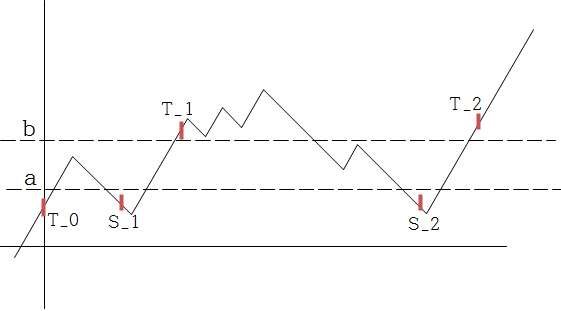
\includegraphics[scale=0.5]{upcrossing}
	\centering
\end{figure}


\thmnum{2.3.1.}(Doob's upcrossing inequality) Let $X$ be a \emph{super-martingale}. Then
\begin{align*}
(b-a) \avg[U[a,b]] \leq \sup_{n\geq 0} \avg[(X_n-a)^{-}]
\end{align*}
(Recall, $x^- = (-x) \vee 0$)
\s

In fact, in this theorem, we prove $(b-a) \avg[U_n[a,b]] \leq  \avg[(X_n-a)^{-}]$.
\begin{proof}
\pf Set $T_0 =0$ and define recursively for $k\geq 0$,
\begin{align*}
S_{k+1} = \inf \{m\geq T_k : X_m <a \}, \quad T_{k+1} = \sup \{m\geq S_{k+1} : X_m >b \}
\end{align*}
Note that if $T_k < \infty$, then $\{S_k, S_{k}+1,\cdots, T_k \}$ is an upcrossing of $[a,b]$ by $X$, and $T_k$ is the time of completion of the $k-th$ upcrossing. Also note that $U_n [a,b] \leq n$. For $m\leq n$, we have
\begin{align*}
\{U_n[a,b] =m \} = \{T_m \leq n < T_{m+1} \}
\end{align*}
On this event,
\begin{align*}
X_{T_k \wedge n}  - X_{S_k \wedge n} = \begin{cases}
X_{T_k} - X_{S_k} \geq b-a \quad \text{if } k\leq m \\
X_n - X_{S_k} \geq X_n -a \quad \text{if } k \geq m+1, S_{m+1} \leq n \\
0 \quad \text{otherwise}
\end{cases}
\end{align*}
Hence
\begin{align*}
\sum_{k=1}^n (X_{T_k \wedge n} - X_{S_k \wedge n}) &\geq (b-a) U_n[a,b] + X_n - a \\
&\geq (b-a)U_n[a,b] -(X_n -a)^-
\end{align*}
Since $X$ is a super-martingale and $T_k \wedge n$ and $S_k \wedge n$ are \emph{bounded stopping times} with $S_k \leq T_k$, by optional stopping theorem, we have
\begin{align*}
\avg (X_{T_k \wedge n})\leq \avg(X_{S_k \wedge n})
\end{align*}
By $\avg(\sum_{k=1}^n (X_{T_k \wedge n} - X_{S_k \wedge n})) \leq 0$ we get
\begin{align*}
(b-a) \avg(U_n[a,b]) \leq  \avg[(X_n-a)^-]
\end{align*}
Apply monotone convergence, with $n\rightarrow \infty$, then we are done.

\eop
\end{proof}
\s

This theorem does not seem to have any significance at the moment, but it will turn out to be important later on.

\subsection*{2.4. Doob's maximal inequalities.}

\quad Define $X_n^* = \sum_{k\geq n} |X_k|$
\s

In the next two theorems, we see that the martingale(or sub-martingale) property allows us to obtain estimates on this $X_n^*$ in terms of expectations for $X_n$.\\
\s

\thmnum{2.4.1} (Doob's maximal inequality) Let $X$ be a \emph{martingale or a non-negative sub-martingale}. Then for all $\lambda \geq 0$,
\begin{align*}
\lambda \prob(X_n^* \geq \lambda) \leq \avg(|X_n|   1_{\{ X_n^*\geq \lambda \}}) \leq \avg(|X_n|)
\end{align*}
\begin{proof}
\pf If $X$ is a martingale, then $|X|$ is a non-negative sub-martingale. It suffices to consider the case where $X$ is a non-negative sub-martingale.

\quad Set $T = \inf \{ k \geq 0 : X_k \geq \lambda \} \wedge n$. Then $T$ is a stopping time and $T\leq n$, so by optional stopping, has
\begin{align*}
\avg(X_n) \geq \avg(X_T) &= \avg(X_T 1_{X^*_n \geq \lambda}) + \avg(X_T 1_{X^*_n < \lambda}) \\
& = \avg( \lambda 1_{X^*_n \geq \lambda})  + \avg(X_n 1_{X_n^* < \lambda})
\end{align*}
and
\begin{align*}
\avg(X_n 1_{X^* \geq \lambda}) \geq \lambda \prob(X^*_n \geq \lambda)
\end{align*}

\eop
\end{proof}
\s

\thmnum{2.4.2} (Doob's $L^p$-inequality) Let $X$ be a \emph{martingale or a non-negative sub-martingale}. Then, for all $p>1$ and $q = p/(p-1)$, we have
\begin{align*}
\norms{X^*_n}{p} \leq q \norms{X_n}{q} 
\end{align*}
\begin{proof}
\pf Again, it suffices to consider when $X$ is a non-negative sub-martingale. Fix $k < \infty$. Then
\begin{align*}
\avg [ (X^*_n \wedge k)^p  ] &= \avg \int_0^k p \lambda^{p-1} 1_{\{x^*_n \lambda \}} d\lambda \quad \text{(integration by parts)}\\
& = \int_0^k p \lambda^{p-1} \prob(X^*_n \geq \lambda) d\lambda \quad \text{(Fubini)} \\
& \leq \int+0^k p\lambda^{p-2} \avg (X_n 1_{X^*_n \geq \lambda}) d\lambda \quad \text{(Doob's maximal inequaltiy)} \\
& =\frac{p}{p-1} \avg(X_n (X^*_n \wedge k)^{p-1} ) \\
& \leq q \norms{X_n}{p} \norms{X^*_n \wedge k}{p}^{p-1} \quad \text{(H\"{o}lder's inequality)}
\end{align*}
Hence , $\norms{X^*_n \wedge k}{p} \leq q\norms{X_n}{p}$. Apply monotone convergence theorem with $k\rightarrow \infty$, then we have the desired result.

\eop
\end{proof}
\s

Doob's maximal and $L^p$ inequalities have different versions which apply under the same hypothesis to
\begin{align*}
X^* = \sum_{n\geq 0} |X_n|
\end{align*}
since $X^*_n \nearrow X^*$. Letting $n\rightarrow \infty$ in Doob's maximal inequality gives
\begin{align*}
\lambda \prob(X^* \geq \lambda) \lim_{n\rightarrow \infty} \lambda \prob(X^*_n \geq \lambda) \leq \sup_{n\geq 0} \avg(|X_n|)
\end{align*}
We can then replace $\lambda \prob(X^* >\lambda)$ by $\lambda \prob (X^* \geq \lambda)$ by taking limits from the right in $\lambda$.

\quad Similarly, for $p\in (1,\infty)$ by monotone convergence,
\begin{align*}
\norms{X^*}{p} \leq q \sup_{n\geq 0} \norms{X_n}{p}
\end{align*}
\s

\newday

(19th October, Friday)
\s

\subsection*{2.5. Doob's martingale convergence theorems}

We are going to study three different martingale convergence theorems. They are all important.
\s

\begin{itemize}
\item We say that a random process $X$ is \textbf{$L^p$-bounded} if $\sum_{n\geq 0} \norms{X_n}{p} <\infty$.
\item We say that $X$ is \textbf{uniformly integrable} if
\begin{align*}
\sup_{n\geq 0} \avg (| X_n | 1_{|X_n| >\lambda})\rightarrow 0 \quad \text{as }\lambda \rightarrow \infty
\end{align*}
\item If $X$ is $L^p$ bounded for some $p>1$, then this implies that $X$ is uniformly integrable. This again implies that $X$ is $L^1$ bounded. The first implication follows from H\"{o}lder inequality. The second implication is true because $\avg(|X_n|) = \avg(|X_n|1_{|X_n|\leq \lambda} ) + \avg(|X_n|1_{|X_n|> \lambda} ) \leq \lambda + \avg(|X_n|1_{|X_n|> \lambda} )$.
\end{itemize}
\begin{center}
\bluebox{$X$ is $L^p$-bounded, $p>1$}
\vspace{5pt}

$\Downarrow$
\vspace{5pt}

\bluebox{$X$ is Uniformly integrable}
\vspace{5pt}

$\Downarrow$
\vspace{5pt}

\bluebox{$X$ is $L^1$-bounded}
\end{center}
\s

\thmnum{2.5.1}\emph{(Almost sure martingale convergence theorem)} Let $X$ be an \emph{$L^1$-bounded super-martingale}. Then there exists an integrable and $\F_{\infty}$-measurable random variable $X_{\infty}$ such that
\begin{align*}
X_n \rightarrow X \quad \text{\emph{a.s.} as } n\rightarrow \infty
\end{align*}
\begin{proof}
\pf For a sequence of real numbers $(x_n)_{n\geq 0}$, as $n\rightarrow \infty$, $(x_n)_n$ either converges \emph{or} $|x_n|\rightarrow \infty$, \emph{or} $\liminf_{n} x_n < \limsup_{n} x_n$. In the last case, since the rationals are dense in $\reals$, there exist $a,b\in \mathbb{Q}$ such that $\liminf x_n < a<b \limsup x_n$. 

\quad Set $\Omega_0 = \Omega_{\infty} \cap (\bigcap_{a,b\in \mathbb{Q},a<b} \Omega_{a,b})$ where $\Omega_{\infty} = \{ \liminf |X_n| <\infty \}$, $\Omega_{a,b} = \{ U[a,b] < \infty \}$ (Recall that $U[a,b]$ is the number of upcrossings). Then $X_n(\omega)$ converges for all $\omega \in \Omega_0$. By Fatous' lemma,
\begin{align*}
\avg(\liminf |X_n|) \leq \liminf \avg |X_n| <\infty
\end{align*}
so this implies $\prob (\Omega_{\infty}) =1$. By Doob's inequality, for $a<b$, has
\begin{align*}
(b-a) \avg(U[a,b]) \leq |a| + \sup_{n\geq 0} \avg |X_n | <\infty
\end{align*}
and therefore $\prob(\Omega_{a,b})=1$. Putting this together, we deduce that $\prob(\Omega_0) =1$, and we can find a random variable $X_{\infty}$ defined by
\begin{align*}
X_{\infty} = \lim_{n\rightarrow \infty} X_n 1_{\Omega_0}
\end{align*}
Then $X_n\rightarrow X_{\infty}$ a.s. Also $X_{\infty}$ is $\F_{\infty}$-measurable and $|X_{\infty}| \leq \liminf|X_n|$ so $\avg(|X_{\infty}|) <\infty$. Hence $X_{\infty}$ is integrable.

\eop
\end{proof}
\s

\textbf{Remark :} Every non-negative integrable super-martingale is $L^1$-bounded, hence it converges a.s.
\s

\thmnum{2.5.2}\emph{($L^1$ martingale convergence theorem)} Let $(X_n)_{n\geq 0}$ be a \emph{uniformly integrable martingale}. Then there exists a random variable $X_{\infty} \in L^1(\F_{\infty})$ such that
\begin{align*}
X_n \xrightarrow{n\rightarrow \infty} X_{\infty} \quad \text{a.s. and in }L^1
\end{align*}

Moreover, $X_n = \avg(X_{\infty} |\F_n)$ a.s. for all $n\geq 0$.

\quad Conversely, for all $Y\in L^1(\F_{\infty})$, on choosing  version $X_n$ of $\avg(Y|\F_n)$ for all $n$, we obtain a uniformly integrable martingale $(X_n)_{n\geq 0}$ such that
\begin{align*}
X_n \xrightarrow{n\rightarrow \infty} Y \quad \text{a.s. and in }L^1
\end{align*}
\s

We can think of this theorem as establishing the bijection
\begin{center}
\bluebox{unif. integrable martingale/a.s.} $\leftrightarrow$ \bluebox{$L^1(\F_{\infty})$}
\end{center}

\begin{proof}
\pf Let $(X_n)_{n\geq 0}$ be a uniformly integrable martingale. By the almost sure martingale convergence theorem, there exists $X_{\infty} \in L^1(\F_{\infty})$ s.t. $X_n \rightarrow X_{\infty}$ a.s. Since $X$ is uniformly integrable, it also follows that $X_n \rightarrow X_{\infty}$ in $L^1$.(see PM, Thm 2.5.1. and 6.2.3.)

\quad Next, for $m\geq n$,
\begin{align*}
\norms{X_n - \avg(X_{\infty} |\F_{n})}{1} &= \norms{ \avg(X_m-X_{\infty} |\F_n ) }{1} \\
&= \norms{X_m - X_{\infty}}{1} \rightarrow 0 \quad \text{as } m\rightarrow \infty
\end{align*}
Hence $X_n = \avg(X_{\infty} |\F_n)$ a.s.
\s

\quad For the converse statement, suppose $Y\in L^1(\F_{\infty})$ and let $X_n$ be a version of $\avg(Y|\F_n)$ for all $n$. Then $(X_n)_{n\geq 0}$ is a martingale by the tower property, and is uniformly integrable by \textbf{Lemma 1.5.1.} Hence there exists $X_{\infty} \in L^1(\F_{\infty})$ such that $X_n \rightarrow X_{\infty}$ a.s. and in $L^1$. For all $n \geq 0$ and all $A\in \F_{n}$, we have 
\begin{align*}
\avg(X_{\infty} 1_A) = \lim_{m\rightarrow \infty} \avg(X_m 1_A) = \lim_{n\leq m\rightarrow \infty} \avg(\avg(Y 1_A |\F_m)) = \avg(Y1_A)
\end{align*}
where the second equality follows because $\avg(X_m |\F_n) = \avg(Y |\F_n)$. Now $X_{\infty}$, $Y\in L^1(\F_{\infty})$ and $\cup_n \F_n$ is a $\pi$-system generating $\F_{\infty}$. Hence, by Dynkin's lemma,
\begin{align*}
X_{\infty} = Y \quad \text{a.s.}
\end{align*}

\eop
\end{proof}
\s

\thmnum{2.5.3}\emph{($L^p$-martingale convergence theorem)} Let $p\in (1,\infty)$. Let $(X_n)_{n\geq 0}$ be an $L^p$-bounded martingale. Then there exists a random variable $X_{\infty} \in L^p (\F_{\infty})$ s.t.
\begin{align*}
X_n \rightarrow X_{\infty} \quad \text{a.s. and in } L^p
\end{align*}
Moreover, $X_n = \avg(X_{\infty}|\F_n)$ a.s. for all $n\geq 0$.

\quad Conversely, for all $Y\in L^p(\F_{\infty})$, on choosing a version $X_n$ of $\avg(Y|\F_n)$ for all $n$, we obtain an $L^p$-bounded martingale such that $X_n \rightarrow Y$ a.s. and in $L^p$.
\s

This is very similar to the statement of $L^1$-martingale convergence theorem. Indeed, the proof is also very similar.
\begin{proof}
\pf Let $(X_n)$ be an $L^p$-bounded martingale. By \emph{a.s. martingale convergence theorem}, there exists $X_{\infty} \in L^1(\F_{\infty})$, $X_n\rightarrow X_{\infty}$ a.s.

\quad By \emph{Doob's $L^p$-inequality}, $\norms{X^*}{p} \leq q \sup_{n\geq 0} \norms{X_n}{p} < \infty$, where $X^* = \sup_{n\geq 0} |X_n|$. Also, since $|X_n - X_{\infty}|^p \leq (2 X^*)^p$ for all $n$, we may apply dominated convergence theorem to deduce that $X_n \rightarrow X_{\infty}$ in $L^p$. Then $X_n = \avg(X_{\infty} |\F_n)$ a.s. for all $n$, as in the $L^1$-convergence.
\s

\quad For the converse statement, suppose $Y\in L^p(\F_{\infty})$ and let $X_n$ be a version of $\avg(Y|\F_n)$. Then $(X_n)_{n\geq 0}$ is a martingale by the tower property and by Jensen inequality,
\begin{align*}
\norms{X_n}{p} = \norms{\avg(Y|\F_n)}{p} \leq \norms{Y}{p}
\end{align*}
Let $X_n \rightarrow X_{\infty}$ a.s. and in $L^P$ for $X_{\infty} \in L^{p}(\F_{\infty})$, using the previous part. Then proceed as in the proof of $L^1$-convergence to prove that in fact $Y = X_{\infty}$ a.s. 

\eop
\end{proof}
\s

\newday

(22nd October, Monday)
\s

Recall that, for a stopping time $T$ and a random process $X$, $X_T$ has been defined only on $\{T<\infty \}$. Given an almost sure limit $X_{\infty}$ for $X$, we define $X_T = X_{\infty}$ on $\{T= \infty \}$. Then the optional stopping theorem extends to all stopping times for uniformly integrable martingales.
\s

\thmnum{2.5.5.} Let $X$ be a uniformly integrable martingale and let $T$ be any stopping time. Then $\avg(X_T) = \avg(X_0)$. Moreover, for all stopping time $S$ and $T$, we have
\begin{align*}
\avg(X_T |\F_S) = X_{S\wedge T} \quad \text{a.s.}
\end{align*}
\s

This theorem is an extension of Optional stopping theorem, \textbf{Theorem 2.2.2} and \textbf{Theorem 2.2.3}.
\begin{proof}
\pf By the optional stopping time theorem and \textbf{2.2.3}, when applied to the bounded stopping time $T\wedge n$, we have
\begin{align*}
& \avg(X_{T\wedge n}) = \avg(X_0) \\
& \avg(X_{T\wedge n}|\F_S) = X_{S\wedge T\wedge n}
\end{align*}
In order to get the claim by letting $n\rightarrow \infty$, we need to prove $X_{T\wedge n} \rightarrow X_T$ \emph{a.s.} and in $L^1$. This will imply that
\begin{align*}
\avg(X_{T\wedge n}|\F_S) \rightarrow \avg(X_{T}|\F_S) \quad \text{in } L^1
\end{align*}
\begin{subproof}
\textbf{Claim :} $X_{T\wedge n} \rightarrow X_T$ \emph{a.s.} and in $L^1$

\pf By the $L^1$ martingale convergence theorem, there exists $X_{\infty} \in L^1(\F_{\infty})$ s.t. $X_n \rightarrow X_{\infty}$ a.s. and in $L^1$ and $X_n = \avg(X_{\infty}|\F_n)$. This implies $X_{T\wedge n}\rightarrow X_T$ \emph{a.s.} as $n\rightarrow \infty$.(if $T<\infty$, the convergence trivial, and in the case $T=\infty$, the convergence justified the previous statement). Since $F_{T\wedge n} \subset F_n$, by \textbf{Theorem 2.2.3.} and the tower property we have
\begin{align*}
X_{T\wedge n} = \avg(X_n | \F_{T\wedge n})= \avg(X_{\infty}|\F_{T\wedge n})
\end{align*}
By \textbf{Lemma 1.5.1}, $(X_{T\wedge n})_{n\geq 0}$ is uniformly integrable. Hence
\begin{align*}
X_{T\wedge n} \rightarrow X_T \quad \text{in } L^1
\end{align*}
\end{subproof}

\eop
\end{proof}
\s

\subsubsection*{Backward martingale}
\begin{itemize}
\item A \textbf{backward filtration} $(\hat{\F}_n)_{n\geq 0}$ is a sequence of $\sigma$-algebras such that $\F \supset \hat{\F}_n \supset \hat{\F}_{n+1}$.
\item This also defines $\hat{\F}_{\infty} = \bigcap_{n\geq 0} \hat{\F}_n$
\end{itemize}
\s

\thmnum{2.5.4.} \emph{(Backward martingale convergence theorem)} For all $Y\in L^1(\F)$, we have 
\begin{align*}
\avg(Y|\hat{\F}_n) \rightarrow \avg(Y|\hat{\F}_{\infty}) \quad \text{a.s. and in } L^1 \quad \text{as } n\rightarrow \infty
\end{align*}
\s

Note that we do not need a uniformly integrability condition, because our assumption of backward filtration already implies uniform convergences.
\begin{proof}
\pf Write $X_n = \avg(Y|\hat{\F}_n)$ for all $n\geq 0$. Fix $n\geq 0$, by the Tower property, $(X_{n-k})_{0\leq k\leq n}$ is a martingale for the filtration $(\hat{\F}_{n-k})_{0\leq k\leq n}$. For $a<b$, the number $U_n[0,\infty]$ of upcrossings of $[a,b]$ by $(X_k)_{0\leq k \leq n}$ equals the number of upcrossings of $[-b,-a]$ by the process $(-X_{n-k})_{0\leq k\leq n}$. Hence by (the note on) \textbf{Theorem 2.3.1},
\begin{align*}
(b-a)\avg(U_n [a,b]) \leq \avg((X_0 -b)^+)
\end{align*}
and so by monotone convergence,
\begin{align*}
(b-a) \avg(U[a,b]) \leq \avg((X_0-b)^+) \leq \avg(|X|) + |b| \leq \avg(|Y|) + |b| <\infty
\end{align*}
where the third inequality follows because of Jensen's inequality. Also, 
\begin{align*}
\avg(\liminf |X_n|) \leq \liminf \avg|X_n| \leq \avg|Y| < \infty
\end{align*}
With these properties in hand, we can apply the same proof used to prove almost sure martingale convergence theorem to show that $\prob(\hat{\Omega}_0)=1$, where $\hat{\Omega}_0 = \{X_n$ converges as $n\rightarrow \infty \}$ - observe that $\hat{\Omega}_0 = \{\liminf_n |X_n| < \infty\} \cap (\bigcap_{a,b\in \mathbb{Q},a<b} \{ U[a,b]<\infty  \} )$ and we see that each set in the intersection has measure 1, and therefore $\prob(\hat{\Omega}_0)=1$.

\quad Set $X_{\infty} = 1_{\hat{\Omega}_0} \lim_{n\rightarrow \infty} X_n$. Then $X_{\infty} \in L^1(\hat{\F}_{\infty})$ and $X_n \rightarrow X_{\infty}$ a.s. Now $(X_n)_{n\geq 0}$ is uniformly integrable (by \textbf{Lemma 1.5.1}), so $X_n\xrightarrow{L^1} X_{\infty}$. Finally, for all $A\in \hat{F}_{\infty}$, we have
\begin{align*}
\avg((X_{\infty} - \avg(Y|\hat{\F}_{\infty})) 1_A) = \lim_{n\rightarrow \infty} \avg((X_n -Y)1_A) = 0
\end{align*}
This implies $X_{\infty} = \avg(Y|\hat{\F}_{\infty})$ a.s.

\eop
\end{proof}

\section*{3. Applications of martingale theory}

\subsection*{Sums of independent random variables}

\newcommand{\T}{\mathscr{T}}

Let $S_n = X_1 + \cdots + X_n$, where $(X_n)_{n\geq 0}$ is a sequence of independent random variables.
\s

\thmnum{3.1.1} \emph{(Strong Law of Large Numbers)} Let $(X_n)_{n\geq 0}$ be a sequence of independent identically distributed (\emph{i.i.d}) integrable random variables. Set $\mu = \avg(X_{1})$. Then
\begin{align*}
S_n / n \rightarrow \mu \quad \text{ a.s. and in } L^1
\end{align*}
\begin{proof}
\pf Define $\hat{\F}_n = \sigma(S_m : m\geq n)$, $\T_n = \sigma(X_m : m\geq n+1)$ and $\T = \cap_{n\geq 1} \T_n$. Then $\hat{\F}_n = \sigma(S_n, \T_n)$ and $(\hat{\F}_n)_{n\geq 1}$ is a backward filtration. Since $\sigma(X_1, S_n)$ is independent of $\T_n$, we have
\begin{align*}
\avg(X_1 |\hat{\F}_n) = \avg(X_1 |S_n) \quad \text{a.s.}
\end{align*} 
For $k\leq n$ and all Borel sets $B$, we have
\begin{align*}
\avg(X_k 1_{ \{S_n \in B \} }) = \avg(X_1 1_{\{S_n \in B \} })
\end{align*}
by symmetry $(X_k, S_n) \xeq (X_1, S_n)$ in distribution, so $\avg(X_k | S_n) = \avg(X_1 |S_n)$ a.s. But
\begin{align*}
\avg(X_1 |S_n)+ \cdots + \avg(X_n|S_n) = \avg(S_n |S_n) = S_n \quad \text{a.s.}
\end{align*} 
so $\avg(X_1 |\hat{\F}_n) = S_n /n$ almost surely. Then by backward martingale convergence theorem, has $S_n/n\rightarrow Y$ a.s. and in $L^1$ for some random variable $Y$. Then $Y\in \T$. By Kolmogorov's 0-1 law [PM \textbf{Theorem 2.6.1}], $Y$ is almost surely a constant. Hence
\begin{align*}
Y = \avg(Y) = \lim \avg(S_n/n) = \mu \quad \text{a.s.}
\end{align*}
where the second equality follows from $L^1$ convergence $S_n/n\rightarrow Y$.

\eop
\end{proof}
\s

Since a.s. convergence implies convergence in probability, we have the following corollary.
\s

\corrnum{3.1.2} \emph{(Weak law of large numbers)} Let $(X_n)_{n\geq 1}$ be a sequence of i.i.d. integrable r.v.. Set $\mu =\avg(X_1)$. Then 
\begin{align*}
\prob(|\frac{S_n}{n} -\mu| > \epsilon) \rightarrow 0 \quad \text{as } n\rightarrow \infty \quad \forall \epsilon >0
\end{align*}
\s

\newday

(24th October, Wednesday)
\s

\subsection*{3.2. Non-negative martingale and change of measure}
\newcommand{\nprob}{\tilde{\prob}}

\begin{itemize}
\item Given a random variable $X$, $\F$-measurable with $X\geq 0$ and $\avg(X) =1$, we can define a new probability measure for $\tilde{\prob}$ on $\F$ by
\begin{align*}
\tilde{\prob}(A) = \avg(X1_A) \quad \forall A\in \F
\end{align*}
Moreover, by [PM, Prop 3.1.4], given $\nprob$, this equation determines $X$ uniquely, up to a.s. modification. We say \textbf{$\nprob$ has a density w.r.t. $\prob$} and $X$ is a version of the density.
\item Let $(\F_n)_{n\geq 0}$ be a filtration in $\F$ and assume $\F = \F_{\infty}$. Let $(X_n)_{n\geq 0}$ be an adapted random process, with $X_n \geq 0$ and $\avg(X_n) =1$ for all $n$. We can define, for each $n$, a new probability measure $\nprob_n$ on $\F_n$ by
\begin{align*}
\nprob_n (A) = \avg(X_n 1_A) \quad \forall A\in \F_n
\end{align*}
Since we require each $X_n$ to be $\F_n$-measurable, this equation determines $X_n$ uniquely up to a.s. modification. 
\end{itemize}
\s

\propnum{3.2.1.} The measures $\nprob_n$ are consistent. That is
\begin{align*}
\nprob_{n+1} | \F_n = \nprob_n \quad \forall n \quad \text{\emph{iff}} \quad (X_n)_{n\geq 0} \quad \text{is a martingale}
\end{align*}
Moreover, there is a measure $\nprob$ on $\F$, which has a density w.r.t $\prob$ such that
\begin{align*}
\nprob |\F_n = \nprob_n \quad \forall n \quad \text{\emph{iff}} \quad (X_n)_n \quad \text{is a uniformly integrable martingale}
\end{align*}
\begin{proof}
\pf (The proof was an exercise.)
For the first point,
\begin{align*}
\nprob_n (A) = \nprob_{n+1}(A |\F_n) = \avg(X_{n+1} 1_A |\F_n) = \avg(X_{n+1}|\F_n) 1_A  \quad \forall A \in \F_n \\
\Leftrightarrow \quad \avg(X_{n+1} |\F_n) = X_n \quad \text{a.s.} \quad \Leftrightarrow \quad (X_n) \text{ is a martingale}
\end{align*}

\quad For the second point, suppose $\nprob |\F_n = \nprob_n \quad \forall n$. Then $\nprob_n |\F_m  =(\nprob | \F_n) | \F_m = \nprob_m$ whenever $n\geq m$, so we find that $(X_n)_n$ is a martingale. Since we assumed that $\avg(X_n)=1$ for all $n$, by almost everywhere martingale convergence theorem, we find a random variable $X$ such that $X_n \rightarrow X$ a.s. Now for any $A \in \F$, we may find $N \geq 0$ such that $A\in \F_k$ for all $k\geq N$, so
\begin{align*}
\nprob(A) = \nprob(A |\F_k) = \nprob_k (A) = \avg(X_k 1_A) \xrightarrow{k\rightarrow \infty} \avg(X 1_A)
\end{align*}
and therefore $\nprob(A) = \avg(X 1_A)$. Hence for all $n \geq 0$, we have
\begin{align*}
\avg(X 1_A|\F_n) = \nprob(A |\F_n) = \avg(X_n 1_A) \quad \forall A \in \F_n
\end{align*} 
and therefore $X_n = \avg(X|\F_n)$. This shows that $(X_n)_n$ is uniformly integrable martingale.

\quad For the converse direction, assume that $(X_n)_n$ is uniformly integrable. Then by $L^1$-martingale convergence theorem, we may find $X \in \F_{\infty}$ such that $X_n \rightarrow X$ in $L^1$ and a.s. Define $\nprob(A) = \avg(X 1_A)$. Then $\nprob(A |\F_n) = \avg(\avg(X 1_A |F_n)) = \avg(X_n 1_A)$ for any $n\geq 0$ and $A\in \F_n$, and therefore $\nprob | \F_n = \nprob_n$. 

\eop 
\end{proof}
\s

\thmnum{3.2.3} \emph{(Radon-Nikodym theorem)} Let $\mu$ and $\nu$ be $\sigma$-finite measures on a measurable space $(E, \mathscr{E})$. Then the followings are equivalent :
\begin{itemize}
\item[(a)] $\nu(A) =0$ for all $A\in \mathscr{E}$ such that $\mu(A) =0$, i.e. $\nu$ is \textbf{absolutely continuous} with respect to $\mu$.
\item[(b)] There exists a measurable function $f$ on $E$ such that $f\geq 0$ and $\nu(A) = \mu(f 1_A)$ for all $A\in \mathscr{E}$.
\end{itemize}
\s

The function $f$ which is unique up to modification $\mu$-a.e. is called (a version of) the \textbf{Radon-Nikodym derivative} of $\nu$ with respect to $\mu$. We write $f = d\nu /d\mu$ almost surely. 
\s

We will give a proof for the case \emph{where $\mathscr{E}$ is countably generated}. We assume there is a sequence $(G_n : n \in \mathbb{N})$ of subsets of $E$ which generates $\mathscr{E}$. This holds, for example, whenever $\mathscr{E}$ is the Borel $\sigma$-algebra. of a topology with countable basis. A further martingale argument is required to prove the general case, but we omit it.
\begin{proof}
\pf The direction (b) $\Rightarrow$ (a) is obvious. So we aim to prove (a) $\Rightarrow$ (b)

\quad By assumption, there is a countable partition of $E$ by measurable sets on which both $\mu$ and $\nu$ are finite. (since $\mu,\nu$ are $\sigma$-finite.) It suffices to show (b) holds on each of these sets, so we can reduce to the case where $\mu$, $\nu$ are finite.

\quad The case $\nu(E) =0$ is clear, as we can just take $f\equiv 0$. So assume $\nu(E) >0$. Then $\mu(E)>0$ by (a). Write $\Omega = E$ and $\F = \mathscr{E}$ and consider the probability measures
\begin{align*}
\prob = \mu / \mu(E) \quad \text{and} \quad \nprob = \nu/\nu(E) \quad \text{on } (\Omega, \F)
\end{align*}
It will suffice to show that there is a random variable $X \geq 0$ such that $\nprob(A) = \avg(X 1_A)$ for all $A\in \F$.

\quad Set $\F_n = \sigma(G_k : k\leq n)$. There exists $m \in \mathbb{N}$ and a partition of $\Omega$ by events $A_1, \cdots, A_m$ such that $\F_n = \sigma (A_1, \cdots, A_m)$ (e.g. choose $A_1 = G_1$, $A_2 = G_2 \backslash G_1$, $A_3 = G_3\backslash (G_1 \cup G_2)$ and so on). Set 
\begin{align*}
X_n = \sum_{j=1}^m a_{j} 1_{A_j}
\end{align*}
where $a_j = \nprob(A_j) / \prob(A_j)$ if $\prob(A_j)>0$ and $a_j =0$ otherwise. Then $X_n \geq 0$, $X_n \in \F_n$.

\quad Observe that $(\F_n)_{n\geq 0}$ is a filtration and $(X_n)_{n\geq 0}$ is a non-negative martingale adapted to $(\F_n)_{n\geq 0}$(has to check this). We will show that $(X_n)_{n\geq 0}$ is \emph{uniformly integrable}. Once shown this, by the $L^1$-martingale convergence theorem, there exists $X\geq 0$ such that $\avg(X 1_A) = \avg(X_n 1_A)$ for all $A \in \F_n$. Define a probability measure $\mathbb{Q}$ on $\F$ by
\begin{align*}
\mathbb{Q}(A) = \avg(X 1_A) \quad \forall A \in \F
\end{align*}
Then $\mathbb{Q} = \nprob$ on $\cup_n \F_n$ which is a $\pi$-system generating $\F$. Hence $\mathbb{Q} = \nprob$ on $\F$, by uniqueness of extension.[PM, Thm 1.7.1], which implies (b).

\quad It remains to show that $(X_n)_n$ is uniformly integrable. Given $\epsilon >0$, we can find $\delta >0$ such that $\nprob(B) <\epsilon$ for all $B \in \F$ with $\prob (B) <\delta$.(If not, there would be a sequence of sets $(B_n)_{n} \subset \F$ with $\prob(B_n)<2^{-n}$ and $\nprob(B) \leq \epsilon$ for all $n$. Then by Borel-Cantielli lemma, $\prob(\limsup B_n) =0$, but $\nprob(\limsup B_n) >\epsilon$, which contradicts (a)). Set $\lambda = 1/\delta$. Then by Markov inequality,
\begin{align*}
\prob(X_n > \lambda) \leq \frac{\avg(X_n)}{\lambda} = \frac{1}{\lambda} = \delta \quad \forall n
\end{align*}
so $\avg(X_n 1_{X_n > \lambda}) = \nprob(X_n > \lambda) < \epsilon$ for all $n$. Hence $(X_n)_n$ is uniformly integrable by its definition

\eop
\end{proof}
\s

\newday

(26th October, Friday)
\s

\subsection*{3.3. Markov Chains}

\begin{itemize}
\item Let $E$ be a \emph{countable set}. We identify each measure $\mu$ on $E$ with $(\mu_x : x\in E)$ where $\mu_x = \mu(\{x\})$. Then for each function $f$ on $E$ write
\begin{align*}
\mu(f) = \mu f = \sum_{x\in E} \mu_x f_x \quad \text{(vector product)}
\end{align*}
where $f_x = f(x)$.
\item A \textbf{transition matrix} on $E$ is a matrix $P=(p_{xy}:x,y\in E)$ such that each row $(p_{xy}:y\in E)$ is a probability measure.
\item Given a filtration $(\F_n)_{n\geq 0}$ and $(X_n)_{n\geq 0}$, and adapted process with values in $E$, we say that $(X_n)_{n\geq 0}$ is a \textbf{Markov chain with transition matrix $P$} if, for all $n\geq 0$, all $x,y\in E$ and all $A\in \F_n$ with $A\subset \{x_n =x \}$ and $\prob(A)>0$,
\begin{align*}
\prob(X_{n+1} =y |A) = p_{xy}
\end{align*}
\end{itemize}
Our notion of Markov chain depends on the choice of $(\F_n)_n$. The following results show that our definition agrees with the usual one with the choice of the natural filtration of $(X_n)_n$.
\s

\propnum{3.3.1} Let $(X_n)_{n\geq 0}$ be a random process in $E$ and take $\F_n = \sigma (X_k : k\geq n)$. Then the following are equivalent :
\begin{itemize}
\item[(a)] $(X_n)_{n\geq 0}$ is a Markov chain with initial distribution $\mu$ and transition matrix $P$.
\item[(b)] For all $n$ and all $x_0,x_1,\cdots,x_n\in E$,
\begin{align*}
\prob(X_0 = x_0, X_1=x_1,\cdots,X_n=x_n) = \mu_{x_0} p_{x_0 x_1} \cdots p_{x_{n-1}x_n}
\end{align*}
\end{itemize}
\s

\propnum{3.3.2} Let $E^*$ denote the set of sequence $x=(x_n : n\geq 0)$ taking values in $E$ and define $X_n : E^* \rightarrow E$ by $X_n(x) = x_n$. Set $\mathscr{E} = \sigma (X_k : k\geq 0)$. Let $P$ be a transition matrix on $E$. Then, for each $y\in E$, there is a unique probability measure $\prob_y$ on $(E^*,\mathscr{E}^*)$ such that $(X_n)_{n\geq 0}$ is a Markov chain with transition matrix $P$ and starting from $y$.
\begin{proof}
\pf The choice of probability measure should be obvious from the transition matrix $P$. To show uniqueness, use Dynkin's lemma.
\end{proof}

\s

An example of a Markov chain in $\mathbb{Z}^d$ is the simple symmetric random walk with transition matrix
\begin{align*}
p_{xy} = \begin{cases}
1/2d \quad \text{if } |x-y| =1 \\
0 \quad \text{otherwise}
\end{cases}
\end{align*}
The following result shows a simple instance of a general relationship between Markov processes and martingale.
\s

\propnum{3.3.3} Let $(X_n)_{n\geq 0}$ be an adapted process in $E$. TFAE :
\begin{itemize}
\item[(a)] $(X_n)_{n\geq 0}$ is a Markov chain with transition matrix $P$.
\item[(b)] For all bounded functions $f$ on $E$, the following process is a \emph{martingale}
\begin{align*}
M^f_n = f(X_n) - f(X_0) - \sum_{k=0}^{n-1} (P-I) f(X_k)
\end{align*}
\end{itemize}
\begin{proof}
\pf (exercise) (Be careful that $(P-I)f(X_n)$ is not $P-I$ applied to $f(X_n)$ but $(P-I)f$ applied to $X_n$.) Suppose that $(X_n)_n$ is a Markov chain. Then
\begin{align*}
& \avg(f(X_{n+1}) |\F_n) = \avg( \sum_{y\in E} f(X_{n+1}) \cha_{X_{n+1}=y} | \F_n) = \sum_{y\in E} f(y) \avg( \cha_{X_{n+1}=y} |\F_n)
\end{align*}
\begin{subproof}
\textbf{Claim :} $\avg(\cha(X_{n+1}=y) |\F_n) = \sum_{x\in X} p_{xy} \cha(X_n = x)$

\pf Observe that $\avg(\cha_{X_{n+1}=y} |\F_n)= \avg\big(\avg(\cha(X_{n+1}=y) |X_n) |\F_n \big)$, so it is sufficient to prove that $\avg(\cha(X_{n+1}=y) |X_n) = \sum_{x\in X} p_{xy} \cha(X_n = x)$. The expression on the right hand side is clearly $\sigma(X_n)$-measurable. Also, for any $A = \{X_n = w\} \in \sigma(X_n)$
\begin{align*}
&\avg( \avg(\cha_{X_{n+1}=y} |X_n)) 1_A ) = \avg( \cha_{X_{n+1}=y} 1_A ) = \prob(X_{n+1}=y, X_n = w) = p_{wy} \prob(X_n =w)
\end{align*}
and
\begin{align*}
\avg(\sum_{x\in X} p_{xy} \cha(X_n = x) 1_A) = \sum_{x\in X}p_{xy} \prob(X_n =x, 1_A) = p_{wy} \prob(X_n = w)
\end{align*}
Since $\{ \{X_n = w\} : w\in E\}$ generates $\sigma(X_n)$, we have the result.
\end{subproof}
Therefore, 
$\avg(f(X_{n+1}) |\F_n) = \sum_{x,y\in E} f(y) p_{xy} 1_{X_n = x} = P(f)(X_n)$ and therefore
\begin{align*}
\avg(f(X_n+1) - f(X_0) - \sum_{k=0}^{n} (P-I) f(X_k) |\F_n) = f(X_n) - f(X_0) - \sum_{k=0}^{n-1} (P-I) f(X_k)
\end{align*}
\s

Now if $(M^f_n)_n$ is a martingale for any bounded function, then it follows that $\avg(f(X_n+1)|X_n) = P(f)(X_n)$ for any bounded $f$ and $n$, and therefore $X_n$ is a Markov chain.
\end{proof}
\s

\begin{itemize}
\item A bounded function $f$ on $E$ is said to be \textbf{harmonic} (for the transition matrix $P$) if 
\begin{align*}
P(f) = f \quad \text{i.e. } \sum_{y\in E} p_{xy}f_y = f_x \quad \forall x\in E
\end{align*}
\item If $f$ is a \emph{bounded harmonic function}, then $(f(X_n))_{n\geq 0}$ is a \emph{bounded martingale.} Then by Doob's convergence theorem, $f(X_n)$ converges a.s. and in $L^p$ for all $p<\infty$.
\item More generally, for $D\subset E$, a \emph{bounded function} $f$ on $E$ is \textbf{harmonic on $D$} if
\begin{align*}
\sum_{y\in E} p_{xy}f_y = f_x \quad \forall x\in D
\end{align*}
\item Let $\partial D = E\backslash D$ and fix a bounded function $f$ on $\partial D$. Set $T= \inf \{n\geq 0: X_n \in \partial D \}$ and define a function $u$ on $E$ by
\begin{align*}
u(x) = \avg_x (f(X_T) 1_{T<\infty} )
\end{align*}
where $E_x$ is the unique probability measure of a Markov chain starting at $x \in E$, as defined in \textbf{Prop 3.3.2}.
\end{itemize}
\s

\thmnum{3.3.4} The function $u$ is bounded, harmonic in $D$, and $u=f$ on $\partial D$. Moreover, if $\prob_x (T<\infty) =1 $ for all $x\in D$, then $u$ is the unique bounded extension of $f$ which is harmonic in $D$.
\begin{proof}
\pf It is clear that $u$ is bounded and $u = f$ on $\partial D$. For all $x,y\in E$ with $p_{xy}>0$ under $\prob_x$, conditional on $\{X_1 = y \}$, $(X_{n+1})_{n\geq 0}$ has distribution $\prob_y$. So for $x\in D$, $u(x)= \sum_{y\in E} p_{xy} u(y)$ showing $u$ is harmonic in $D$.

\quad On the other hand, suppose that $g$ is a bounded function harmonic in $D$ such that $g= f$ on $\partial D$. Then $M = M^g$(where $M$ is as defined in \textbf{Prop 3.3.3}) is a martingale and $T$ is a stopping time, so $M^T$ is also a martingale by optional stopping theorem. But $M_{T \wedge n} = g(X_{T\wedge n})$ so if $\prob_x (T <\infty)=1$ for all $x\in D$, then
\begin{align*}
M_{T \wedge n} \rightarrow g(X_T) = f(X_T) \quad \text{a.s.}
\end{align*}
So by bounded convergence, for all $x\in D$,
\begin{align*}
g(x) = \avg_x (M_0) = \avg_x (M_{T\wedge n}) \rightarrow \avg_x(f(X_T)) = u(x)
\end{align*}
therefore $g(x) = u(x)$ for all $x\in E$.

\eop
\end{proof}
\s

\newday

(29th October, Monday)

\section*{4. Random processes in continuous time}

\subsection*{4.1. Definitions}

\begin{itemize}
\item A \textbf{continuous random process} is a family of random variables $(X_t)_{t\geq 0}$ such that for all $\omega \in \Omega$, the path
\begin{align*}
t \mapsto X_t(\omega) : [0, \infty ) \rightarrow \reals
\end{align*}
is continuous.
\item A function $x:[0, \infty) \rightarrow \reals$ is said to be \textbf{cadlag} if it is \emph{right-continuous with left limits}, \emph{i.e.} for all $t\geq 0$
\begin{align*}
x_s \rightarrow x_t \quad \text{as } s\rightarrow t^+
\end{align*}
and for all $t>$, there exists $x_{t^-} \in \reals$ such that
\begin{align*}
x_s \rightarrow x_{t^-} \quad \text{as } s\rightarrow t^-
\end{align*}
\item A \textbf{cadlag random process} is a family of random variables $(X_t)_{t\geq 0}$ such that for all $\omega \in \Omega$, the path
\begin{align*}
t \mapsto X_t(\omega) : [0, \infty ) \rightarrow \reals
\end{align*}
is cadlag.
\item The space of continuous and cadlag functions on $[0,\infty)$ are denoted $C([0,\infty),\reals)$ and $D([0,\infty), \reals)$ respectively. We equip these spaces with the $\sigma$-algebra generated by the coordinate functions $\sigma (x\mapsto x_t : t\geq 0)$. A continuous(/cadlag) random process $(X_t)_{t\geq 0}$ can then be considered as a random variable $X$ in $C([0,\infty), \reals)$(/$D([0,\infty), \reals)$), given by
\begin{align*}
X(\omega) = (t\mapsto X_t(\omega) : t\geq 0)
\end{align*}
\item The \textbf{finite-dimensional distributions} of a continuous or cadlag process $X$ are the laws $\mu_{t_1, \cdots ,t_n}$ on $\reals^n$ given by $\mu_{t_1,\cdots, t_n}(A) = \prob((X_{t_1},\cdots, X_{t_n}) \in A)$ for $A \in \borel(\reals^n)$ where $n \in \mathbb{N}$ and $0\leq t_1 <\cdots < t_n < \infty$. Since the cylinder sets $\{(X_{t_1}, \cdots, X_{t_n}) \in A\}$ form a generating $\pi$-system, they determine uniquely the law of $X$. We make analogous definition when $\reals$ is replaced by a general topological space.
\end{itemize}

\subsection*{Kolmogorov's Criterion}

\thmnum{4.2.1} \emph{(Kolmogorov's criterion)} Let $p \in (1,\infty)$ and $\beta \in (1/p,1]$. Let $I$ be a dense subset of $[0,1]$ and let $(\xi_t )_{t\in I}$ a family of random variables such that for some constant $C<\infty$,
\begin{align*}
\norms{\xi_s - \xi_t}{p} \leq C|s-t|^{\beta} \quad \forall s,t\in T \quad \quad \cdots\cdots\cdots (\dagger)
\end{align*}
Then there exists a continuous random process $(X_t)_{t\in [0,1]}$ such that $X_t = \xi_t$ \emph{a.s.} for all $t\in I$. Moreover $(X_t)_{t\in [0,1]}$ may be chosen such that for all $\alpha \in [0, \beta - \frac{1}{p})$ such that
\begin{align*}
|X_s - X_t| \leq K_{\alpha} |s-t|^{\alpha} \quad \forall s,t \in [0,1]
\end{align*}
\s

This theorem indicates that $L^p$-H\"{o}lder continuity on a dense subset implies H\"{o}lder continuity of the random process. Later, this becomes important in construction of Brownian motion, and different stochastic processes.
\begin{proof}
\pf For $n \geq 0$, write
\begin{align*}
& \mathbb{D}_n = \{ k2^{-n}  : k \in \mathbb{Z}^+ \} \quad \mathbb{D}= \bigcup_{n\geq 0} \mathbb{D}_n \\
& D_n = \mathbb{D}_n \cap [0,1] \quad D = \mathbb{D} \cap [0,1]
\end{align*}
By taking limits in $L^p$, we can extend $(\xi_t)_{t\in I}$ to all $t\in D$ and such that $(\dagger)$ holds for all $s,t\in D\cup I$.(The limit exist, because each sequence converging to a point forms a Cauchy sequence).

\quad For $n \geq 0$ and $\alpha \in [0, \beta - \frac{1}{p})$, define non-negative random variable by
\begin{align*}
K_n = \sup_{t\in D_n} |\xi_{t+ 2^{-n}} - \xi_t|, \quad K_{\alpha} =2\sum_{n\geq 0} 2^{n\alpha} K_n
\end{align*}
Then
\begin{align*}
\avg((K_n)^p) \leq \avg \Big( \sum_{t\in D_n} |\xi_{t+{2^{-n}}} - \xi_t |^p \Big) \leq 2^n C^p (2^{-n})^{\beta p} \quad (\text{by } (\dagger))
\end{align*}
so
\begin{align*}
\norms{K_{\alpha}}{p} \leq 2 \sum_{n\geq 0} 2^{n\alpha} \norms{K_n}{p} \leq 2C \sum_{n\geq 0} 2^{-(\beta - \alpha - \frac{1}{p})n} < \infty
\end{align*}
For $s,t\in D$, with $s<t$, choose $m\geq 0$ such that $2^{-m-1} <t-s \leq 2^{-m}$. Then interval $[s,t)$ can be expressed as a finite disjoint union of intervals of the form $[r, r+ 2^{-n})$ where $r\in D_n$ and $n\geq m+1$ and no 3 intervals have the same length. Hence $|\xi_t - \xi_s | \leq 2\sum_{n\geq m+1} K_n$ and so 
\begin{align*}
\frac{|\xi_t - \xi_s|}/{(t-s)^{\alpha}} \leq 2\sum_{n\geq m+1} K_n 2^{(m+1)\alpha} \leq K_{\alpha}
\end{align*}
Now define
\begin{align*}
X_t(\omega) = \begin{array}{ll}
\lim_{s\rightarrow t, s\in D} \xi_s (\omega)  & \text{if } K_{\alpha}(\omega) < \infty \text{ for all } \alpha \in [0,\beta -\frac{1}{p}) \\
0 & \text{otherwise}
\end{array}
\end{align*}
but $\prob(K_{\alpha}(\omega) < \infty \text{ for all } \alpha \in [0,\beta -\frac{1}{p})) =1$ (note that $K_{\alpha}$ is an increasing function of $\alpha$, so it is enough to take countable sequence $(\alpha_k)_k\rightarrow \beta -\frac{1}{p}$), so $X_t(\omega) = \lim_{s\rightarrow t}\xi_s(\omega)$ a.s. Then $(X_t)_{t\in [0,1]}$ is a continuous random process with the claimed properties.

\eop
\end{proof}
\s

\subsection*{4.3. Martingales in continuous time}

We assume in this section that our probability space $(\Omega, \F, \prob)$ is equipped with a \textbf{continuous filtration}, \emph{i.e.} a family of $\sigma$-algebras $(\F_t)_{t\geq s}$ such that $\F_s \subset \F$ for all $s\leq t$.

\begin{itemize}
\item Define for $t\geq 0$, $\F_{t^+} = \bigcap_{s>t} \F_s$, $\F_{\infty}  = \sigma(\F_t : t\geq 0)$ and
\begin{align*}
\mathscr{N} = \{A\in \F_{\infty} : \prob(A) =0 \}
\end{align*}
\item The filtration $(\F_t)_{t\geq 0}$ is said to satisfy the \textbf{usual conditions} if $\mathscr{N} \subset \F_{0}$ and $\F_t = \F_{t^+}$ for all $t$.
\item A continuous(/cadlag) adapted integrable random process is said to be a \textbf{martingale} if, for all $s,t\geq 0$ with $s\leq t$,
\begin{align*}
\avg(X_t|\F_s) = X_s \quad \text{a.s.} 
\end{align*}
Define super-martingale and sub-martingale accordingly.
\end{itemize}









\end{document}